\documentclass{beamer}
\beamerdefaultoverlayspecification{<+->}
%
% Choose how your presentation looks.
%
% For more themes, color themes and font themes, see:
% http://deic.uab.es/~iblanes/beamer_gallery/index_by_theme.html
%
\mode<presentation>
{
  \usetheme{default}      % or try Darmstadt, Madrid, Warsaw, ...
  \usecolortheme{default} % or try albatross, beaver, crane, ...
  \usefonttheme{default}  % or try serif, structurebold, ...
  \setbeamertemplate{navigation symbols}{}
  \setbeamertemplate{caption}[numbered]
  \setbeamertemplate{footline}[frame number]
} 

\usepackage[english]{babel}
\usepackage[utf8]{inputenc}
\usepackage[T1]{fontenc}
\usepackage{graphicx}
\graphicspath{ {./images/} }
\usepackage{hyperref}
\usepackage{pgfplots}
\usepackage{float}
\pgfplotsset{compat=1.7}

\hypersetup{
    colorlinks=true,
    linkcolor=blue,
    filecolor=magenta,      
    urlcolor=cyan,
    bookmarks=true,
    pdfpagemode=FullScreen,
    }

\title{Econ 200 Section AJ}
\author{Lukas Hager \\ \href{mailto:lghhager@uw.edu}{lghhager@uw.edu}}
\institute{Office Hours: Monday 8-9, Thursday 3:30-4:30}
\date{February 19, 2021}

\begin{document}

\begin{frame}
  \titlepage
\end{frame}

% Uncomment these lines for an automatically generated outline.
%\begin{frame}{Outline}
%  \tableofcontents
%\end{frame}

\begin{frame}{Your Questions}
    Do you have questions about what you've read in the text or heard in lecture?
\end{frame}

\begin{frame}[t]{Handlebars}
    Last year, Jarod left a job that pays \$60,000 to run his own bike-repair shop. Jarod’s shop charges \$65 for a repair, and last year the shop performed 3,000 repairs. Jarod’s production costs for the year included rent, wages, and equipment. Jarod spent \$50,000 on rent and \$100,000 on wages for his employees. Jarod keeps whatever profit the shop earns, but does not pay himself an official wage. Jarod used \$20,000 of his savings to buy a machine for the business. His savings were earning an annual interest rate of 5 percent.
    \begin{itemize}
        \item What is Jarod's annual accounting profit?
    \end{itemize}
\end{frame}

\begin{frame}[t]{Handlebars}
    Last year, Jarod left a job that pays \$60,000 to run his own bike-repair shop. Jarod’s shop charges \$65 for a repair, and last year the shop performed 3,000 repairs. Jarod’s production costs for the year included rent, wages, and equipment. Jarod spent \$50,000 on rent and \$100,000 on wages for his employees. Jarod keeps whatever profit the shop earns, but does not pay himself an official wage. Jarod used \$20,000 of his savings to buy a machine for the business. His savings were earning an annual interest rate of 5 percent.
    \begin{itemize}
        \item What is Jarod's annual accounting profit?
        \[\begin{split}
            \text{Accounting Profit} &= \text{Revenue} - \text{Explicit Costs} \\
            &=\$65 \times 3,000 - \$100,000 - \$50,000 \\
            &= \$45,000
        \end{split}\]
    \end{itemize}
\end{frame}

\begin{frame}[t]{Handlebars}
    Last year, Jarod left a job that pays \$60,000 to run his own bike-repair shop. Jarod’s shop charges \$65 for a repair, and last year the shop performed 3,000 repairs. Jarod’s production costs for the year included rent, wages, and equipment. Jarod spent \$50,000 on rent and \$100,000 on wages for his employees. Jarod keeps whatever profit the shop earns, but does not pay himself an official wage. Jarod used \$20,000 of his savings to buy a machine for the business. His savings were earning an annual interest rate of 5 percent.
    \begin{itemize}
        \item What is Jarod's annual economic profit?
    \end{itemize}
\end{frame}

\begin{frame}[t]{Handlebars}
    Last year, Jarod left a job that pays \$60,000 to run his own bike-repair shop. Jarod’s shop charges \$65 for a repair, and last year the shop performed 3,000 repairs. Jarod’s production costs for the year included rent, wages, and equipment. Jarod spent \$50,000 on rent and \$100,000 on wages for his employees. Jarod keeps whatever profit the shop earns, but does not pay himself an official wage. Jarod used \$20,000 of his savings to buy a machine for the business. His savings were earning an annual interest rate of 5 percent.
    \begin{itemize}
        \item What is Jarod's annual economic profit?
        \[\begin{split}
            \text{Accounting Profit} &= \text{Revenue} - \text{Explicit Costs} - \text{Implicit Costs}\\
            &=\$65 \times 3,000 - \$100,000 - \$50,000 \\
            &\hspace{5 mm}-\$20,000 \times .05 - \$60,000\\
            &= -\$16,000
        \end{split}\]
    \end{itemize}
\end{frame}

\begin{frame}[t]{Matsuko}
    The table below shows the technology of production at the Matsuko's Mushroom Farm for the month of May.
    \begin{table}[H]
    \centering
    \begin{tabular}{cc}
    Number of Workers & Mushrooms per Day (pounds) \\
    1                 & 12                         \\ \hline
    2                 & 30                         \\ \hline
    3                 & 45                         \\ \hline
    4                 & 50                         \\ \hline
    5                 & 54                         \\ \hline
    6                 & 56                       
    \end{tabular}
    \end{table}
    \begin{itemize}
        \item What is is the marginal product of the 4th worker?
    \end{itemize}
\end{frame}

\begin{frame}[t]{Matsuko}
    The table below shows the technology of production at the Matsuko's Mushroom Farm for the month of May.
    \begin{table}[H]
    \centering
    \begin{tabular}{cc}
    Number of Workers & Mushrooms per Day (pounds) \\
    1                 & 12                         \\ \hline
    2                 & 30                         \\ \hline
    3                 & 45                         \\ \hline
    4                 & 50                         \\ \hline
    5                 & 54                         \\ \hline
    6                 & 56                       
    \end{tabular}
    \end{table}
    \begin{itemize}
        \item What is the average product of labor when the farm hires 5 workers?
    \end{itemize}
\end{frame}

\begin{frame}[t]{Matsuko}
    The table below shows the technology of production at the Matsuko's Mushroom Farm for the month of May.
    \begin{table}[H]
    \centering
    \begin{tabular}{cc}
    Number of Workers & Mushrooms per Day (pounds) \\
    1                 & 12                         \\ \hline
    2                 & 30                         \\ \hline
    3                 & 45                         \\ \hline
    4                 & 50                         \\ \hline
    5                 & 54                         \\ \hline
    6                 & 56                       
    \end{tabular}
    \end{table}
    \begin{itemize}
        \item Diminishing marginal returns sets in when the \underline{\phantom{fifth}} worker is hired.
    \end{itemize}
\end{frame}

\begin{frame}[t]{Fancy}
    Fancy Footwear manufactures shoes. The figure below shows Fancy Footwear's marginal product of labor and average product of labor curves in the short run.
    \begin{center}
        \includegraphics[scale = .6]{images/graph.png}
    \end{center}
    \begin{itemize}
        \item Identify the Marginal Product and the Average Product?
    \end{itemize}
\end{frame}

\begin{frame}[t]{Fancy}
    Fancy Footwear manufactures shoes. The figure below shows Fancy Footwear's marginal product of labor and average product of labor curves in the short run.
    \begin{center}
        \includegraphics[scale = .6]{images/graph.png}
    \end{center}
    \begin{itemize}
        \item For what quantity of labor does production display diminishing returns?
    \end{itemize}
\end{frame}

\begin{frame}[t]{Fancy}
    \begin{center}
        \includegraphics[scale = .6]{images/graph.png}
    \end{center}
    \begin{itemize}
        \item The law of diminishing marginal returns
        \begin{itemize}
            \item sets in because not all workers are equally productive
            \item applies only in the short run
            \item holds even when there are no fixed factors 
            \item ultimately explains why production displays diseconomies of scale
        \end{itemize}
    \end{itemize}
\end{frame}

\begin{frame}[t]{Fancy}
    Fancy Footwear manufactures shoes. The figure below shows Fancy Footwear's marginal product of labor and average product of labor curves in the short run.
    \begin{center}
        \includegraphics[scale = .6]{images/graph.png}
    \end{center}
    \begin{itemize}
        \item In the short run, why does a production function eventually display diminishing returns to labor?
    \end{itemize}
\end{frame}

\begin{frame}{US \& China}
    Why is it that the United States and China use different input combinations to produce a given quantity of cotton and yet, each country produces that quantity at the lowest possible cost?
\end{frame}

\begin{frame}{Foot Massages}
    \scriptsize
    \setlength{\tabcolsep}{1pt}
    \begin{table}[]
    \begin{tabular}{c|c|l|l|l|l|l|l|l}
    \multicolumn{1}{l|}{\begin{tabular}[c]{@{}l@{}}Q of \\ Workers\end{tabular}} & \multicolumn{1}{l|}{\begin{tabular}[c]{@{}l@{}}Q of Foot \\ Massages/Day\end{tabular}} & \begin{tabular}[c]{@{}l@{}}Fixed \\ Cost\end{tabular} & \begin{tabular}[c]{@{}l@{}}Variable \\ Cost\end{tabular} & \begin{tabular}[c]{@{}l@{}}Total \\ Cost\end{tabular} & \begin{tabular}[c]{@{}l@{}}Average \\ Total Cost\end{tabular} & \begin{tabular}[c]{@{}l@{}}Average \\ Fixed Cost\end{tabular} & \begin{tabular}[c]{@{}l@{}}Average \\ Variable Cost\end{tabular} & \begin{tabular}[c]{@{}l@{}}Marginal \\ Cost\end{tabular} \\ \hline
    0                                                                            & 0                                                                                      &                                                       &                                                          &                                                       &                                                               &                                                               &                                                                  &                                                          \\ \hline
    1                                                                            & 10                                                                                     &                                                       &                                                          &                                                       &                                                               &                                                               &                                                                  &                                                          \\ \hline
    2                                                                            & 25                                                                                     &                                                       &                                                          &                                                       &                                                               &                                                               &                                                                  &                                                          \\ \hline
    3                                                                            & 45                                                                                     &                                                       &                                                          &                                                       &                                                               &                                                               &                                                                  &                                                          \\ \hline
    4                                                                            & 60                                                                                     &                                                       &                                                          &                                                       &                                                               &                                                               &                                                                  &                                                          \\ \hline
    5                                                                            & 70                                                                                     &                                                       &                                                          &                                                       &                                                               &                                                               &                                                                  &                                                         
    \end{tabular}
    \end{table}
    \normalsize
    Alicia Gregory owns a foot massage business. She leases 4 computer-controlled massage booths, for which she pays \$125 per day. She cannot increase the number of machines she leases without giving the manufacturer 3 months notice. She can hire as many workers as she wants at a cost of \$75 per day per worker. These are the only two inputs she uses in her business. Use this information to fill in the columns in the above table.
\end{frame}

\begin{frame}{Foot Massages}
    \scriptsize
    \setlength{\tabcolsep}{1pt}
    \begin{table}[]
    \begin{tabular}{c|c|l|l|l|l|l|l|l}
    \multicolumn{1}{l|}{\begin{tabular}[c]{@{}l@{}}Q of \\ Workers\end{tabular}} & \multicolumn{1}{l|}{\begin{tabular}[c]{@{}l@{}}Q of Foot \\ Massages/Day\end{tabular}} & \begin{tabular}[c]{@{}l@{}}Fixed \\ Cost\end{tabular} & \begin{tabular}[c]{@{}l@{}}Variable \\ Cost\end{tabular} & \begin{tabular}[c]{@{}l@{}}Total \\ Cost\end{tabular} & \begin{tabular}[c]{@{}l@{}}Average \\ Total Cost\end{tabular} & \begin{tabular}[c]{@{}l@{}}Average \\ Fixed Cost\end{tabular} & \begin{tabular}[c]{@{}l@{}}Average \\ Variable Cost\end{tabular} & \begin{tabular}[c]{@{}l@{}}Marginal \\ Cost\end{tabular} \\ \hline
    0                                                                            & 0                                                                                      & 500                                                   & 0                                                        & 500                                                   & \infty                                                         & \infty                                                         & \infty                                                            & \infty                                                    \\ \hline
    1                                                                            & 10                                                                                     & 500                                                   & 75                                                       & 575                                                   & 57.5                                                           & 50                                                            & 7.5                                                              & 7.5                                                      \\ \hline
    2                                                                            & 25                                                                                     & 500                                                   & 150                                                      & 650                                                   & 26                                                           & 20                                                            & 6                                                                & 5                                                        \\ \hline
    3                                                                            & 45                                                                                     & 500                                                   & 225                                                      & 725                                                   & 16.11                                                        & 11.11                                                         & 5                                                                & 3.75                                                     \\ \hline
    4                                                                            & 60                                                                                     & 500                                                   & 300                                                      & 800                                                   & 13.33                                                           & 8.33                                                          & 5                                                                & 5                                                        \\ \hline
    5                                                                            & 70                                                                                     & 500                                                   & 375                                                      & 875                                                   & 12.49                                                           & 7.14                                                          & 5.35                                                             & 7.5                                                     
    \end{tabular}
    \end{table}
\end{frame}

\begin{frame}{Foot Massages}
    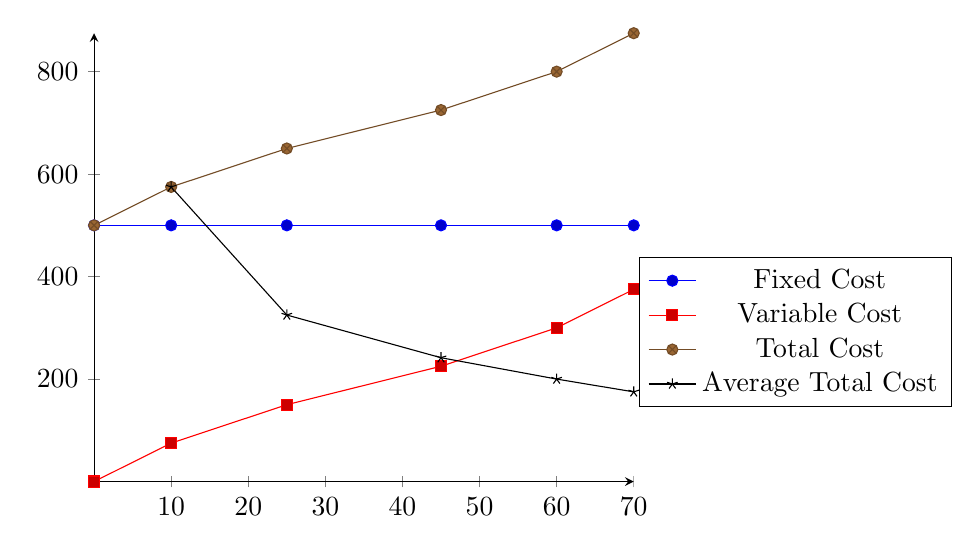
\begin{tikzpicture}
    \begin{axis}[axis lines=center,
    legend style={at={(1.3,.5)},anchor=north}]
    \addplot coordinates {(0,500) (10,500) (25,500) (45,500) (60,500) (70,500)};
    \addlegendentry{Fixed Cost}
    \addplot coordinates {(0,0) (10,75) (25,150) (45,225) (60,300) (70,375)};
    \addlegendentry{Variable Cost}
    \addplot coordinates {(0,500) (10,575) (25,650) (45,725) (60,800) (70,875)};
    \addlegendentry{Total Cost}
    \addplot coordinates {(10,575) (25,325) (45,241.66) (60,200) (70,175)};
    \addlegendentry{Average Total Cost}
    \end{axis}
    \end{tikzpicture}
\end{frame}

\begin{frame}{Foot Massages}
    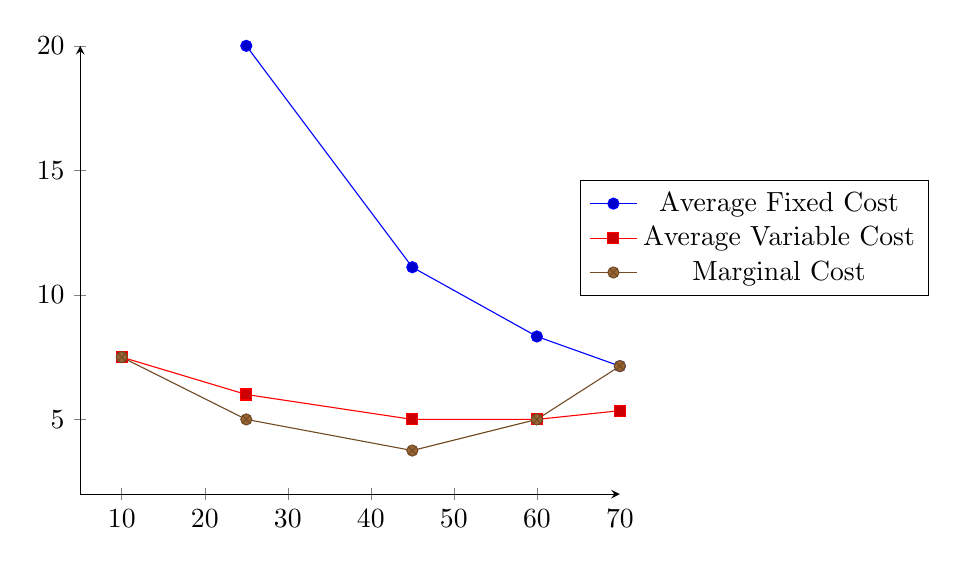
\begin{tikzpicture}
    \begin{axis}[axis lines=center,
    legend style={at={(1.25,.7)},anchor=north}, ymin = 2, xmin = 5]
    \addplot coordinates {(25,20) (45,11.11) (60,8.33) (70,7.14)};
    \addlegendentry{Average Fixed Cost}
    \addplot coordinates {(10,7.5) (25,6) (45,5) (60,5) (70,5.35)};
    \addlegendentry{Average Variable Cost}
    \addplot coordinates {(10,7.5) (25,5) (45,3.75) (60,5) (70,7.14)};
    \addlegendentry{Marginal Cost}
    \end{axis}
    \end{tikzpicture}
    Note that there's a point for AFC at (10,50) that I've omitted here so that you can see the shapes of the curves a little better
\end{frame}

\begin{frame}{Costs Summary}
    \includegraphics[scale = .3]{images/table_costs.png}
\end{frame}

\begin{frame}{Diseconomies of Scale}
    \begin{itemize}
        \item What is the difference between "diminishing marginal returns" and "diseconomies of scale"?
        \begin{itemize}
            \item Diminishing marginal returns happens in the short run when you have at least one fixed factor of production and describes why marginal cost increases after a point
            \item Diseconomies of scale happens in the long run when all factors of production are variable, and describes why average cost increases after a point.
        \end{itemize}
    \end{itemize}
\end{frame}

\begin{frame}{Firms}
    Consider a firm that increases its inputs by 15 percent. For each scenario, state whether the firm experiences economies of scale, diseconomies of scale, or constant returns to scale.
    \begin{itemize}
        \item Outputs increase 15 percent.
        \item Outputs increase by less than 15 percent.
        \item Outputs increase by greater than 15 percent.
    \end{itemize}
\end{frame}

\begin{frame}{Cutler}
    \begin{table}[]
    \begin{tabular}{cc}
    Quantity (Sets) & Long Run Average Cost \\ \hline
    100             & \$40                  \\ \hline
    200             & \$35                  \\ \hline
    300             & \$30                  \\ \hline
    400             & \$30                  \\ \hline
    500             & \$35                 
    \end{tabular}
    \end{table}
    Elegant Settings manufactures stainless steel cutlery.
    \begin{itemize}
        \item Elegant Settings experiences economies of scale at an output of \underline{\phantom{3000}} or less and diseconomies of scale at an output level above \underline{\phantom{4000}}.
        \item What is the minimum efficient scale of production?
        \item Over what range of output does it experience constant returns to scale?
    \end{itemize}
\end{frame}

\end{document}
